
\boxx{
\textbf{Recommended videos}
\tv \textit{Macro: Unit 2.1 -- Aggregate Demand}, siehe: \url{https://youtu.be/AmX0gaLDiPo}\\
\tv \textit{Macro: Unit 2.2 -- Short-Run Aggregate Supply}, siehe: \url{https://youtu.be/GgOttANW0ps}
%\tv \textit{}, siehe: \url{}\\
}


\subsection{The first lockdown at 23 March 2020...}

\dots was a \textbf{shock}


\begin{center}
\includegraphics[width=0.2\textwidth]{/home/sthu/Dropbox/hsf/pic/makro/smiley-shock}
\includegraphics[width=0.2\textwidth]{/home/sthu/Dropbox/hsf/pic/makro/stayhome}
\end{center}

\includegraphics[width=0.23\textwidth]{/home/sthu/Dropbox/hsf/pic/makro/lock3}
\includegraphics[width=0.3\textwidth]{/home/sthu/Dropbox/hsf/pic/makro/lock1}
\includegraphics[width=0.4\textwidth]{/home/sthu/Dropbox/hsf/pic/makro/lock2}

\pbn


\boxb{
%	Der Begriff  stammte ursprünglich aus der Medizin, wo er für den Menschen als lebensbedrohliches Zustandsbild gilt. [...] 
\zitat{\citet[][Entry: Shock (economics)]{Wikipedia2022}:
	``In economics, a shock is an unexpected or unpredictable event that affects an economy, either positively or negatively. Technically, it is an unpredictable change in exogenous factors-that is, factors unexplained by an economic model-which may influence endogenous economic variables.
	
	The response of economic variables, such as GDP and employment, at the time of the shock and at subsequent times, is measured by an impulse response function.''
}
}
%\pbn
\exex{Economic consequences}{
\begin{minipage}{0.25\textwidth}
	\includegraphics[width=0.8\textwidth]{/home/sthu/Dropbox/hsf/pic/makro/covid123}
\end{minipage}
\begin{minipage}{0.75\textwidth}
	Open the link: \webbig \huge https://t1p.de/covid123 \normalsize and list what you consider to be the most important economic effects of the first lockdown. 
\end{minipage}
}


%\includegraphics[width=0.2\textwidth]{pic/nhk}
%\includegraphics[width=0.18\textwidth]{pic/mixtape}

\pbn
\solx{Economic consequences}{
Many things can be mentioned here, for example:
\itex{
	\item -4.9\% in gross domestic product: Economic output collapses significantly in 2020
	\item 4.2 \% deficit ratio: Second-highest government deficit since German unification
	\item 74.5 \% fewer air passengers - lowest figure since German unification
	\item 4.6 \% less consumer spending by private households - sharpest decline in decades
	\item 27.8 \% increase in online retail sales since outbreak of pandemic
	\item 0 \% Population growth in Germany - first since 2011
	\item 21 \% Fewer foreign university entrants in the 2020 academic year
	\item -1.1 \% in real wages - sharpest decline since survey began
	\item 10.7 \% fewer traffic fatalities - lowest level in almost 70 years
	\item 47 \% electricity from renewable energies - a record high
	}\bigskip


Source: \cite{Destatis2021Die}, for more information about the above facts see \websmall \url{https://www.destatis.de/DE/Themen/Querschnitt/Corona/Wirtschaft/kontextinformationen-wirtschaft.html}

and here:
 \websmall \url{https://www.destatis.de/DE/Themen/Querschnitt/Corona/_inhalt.html}
}
\pbn


\includegraphics[width=.9\textwidth]{/home/sthu/Dropbox/hsf/pic/makro/umsatz-gastgewerbe-preise}

\includegraphics[width=.9\textwidth]{/home/sthu/Dropbox/hsf/pic/makro/umsatz_im_kfz-handel}

\includegraphics[width=.9\textwidth]{/home/sthu/Dropbox/hsf/pic/makro/absatz_verbrauchsgueter}

\pbn
\subsection{Value added and price level}

\itex{
\item During the Corona crisis, massive changes occurred in various markets. 
\item The \textbf{gross domestic product} is 
the most important indicator of a country's value added and prosperity, subsumes many different economic effects and is the result of aggregate demand and aggregate supply. 
}

%\subsection*{Der aggregierte Blick:}

\begin{minipage}{0.6\textwidth}
%\begin{figure}
\begin{center}
	\includegraphics[width=.9\textwidth]{/home/sthu/Dropbox/hsf/pic/makro/deu}\label{fig:deu}
\end{center}
%\caption{Preise und BIP in Deutschland von 2017 bis 2021}\ļabel{fig:deu}
%\end{figure}
\end{minipage}
\begin{minipage}{0.4\textwidth}
The \textbf{gross domestic product} indicates the total value of all goods and services produced as final goods and services within the national borders of an economy during one year, after deduction of all intermediate consumption.

The \textbf{price level} is an economic indicator that shows how many monetary units must be paid in an economy for the prices of certain goods and services in a basket of goods.  
\end{minipage}


\pbn
\subsection{How did GDP fall while price levels remained roughly constant?}

\itex{
	\item Less was bought/sold (value added $\downarrow$). 
	\item But why? Was there less demand or were fewer offered?
	\boxb{For example, is the lower hospitality sales the result of guests staying away (demand $\downarrow$), of business closures being ordered (supply $\downarrow$), or of both?}	
	\item Apart from anecdotal evidence, it is difficult to capture all the effects empirically. In markets, usually only the price and the quantity successfully demanded can be observed. 
	\item Solution: Theory $\rightarrow$ The AS-AD Model!
}
%\pbn

\paragraph{General equilibrium}

The interplay of supply and demand determines the equilibrium on the market. 

\begin{center}
	\begin{tikzpicture}[scale=0.3]	
		\draw[thick,<->] (0,9) node[above]{$P$}--(0,0) node[below right]{}--(12,0) node[below]{$Y$};
		\draw(1,1.5) -- (8.5,9) node[above]{$AS$};
		\draw (2,9) --(8.5,1.3) node[right]{$AD$};
		\tkzDefPoint(5,5.5){B}
		\foreach \n in {B}
		\node at (\n)[circle,fill,inner sep=1.5pt]{};
		\draw[dashed](5,5.5)--(5,0) node[below]{$Y^{*}$};
		\draw[dashed](5,5.5)--(0,5.5) node[left]{$P^{*}$};				
		%		\draw(8,9)--(8,0) node[below]{$Y_f$};
		%		\draw[dashed](6.53,3.6)--(6.53,0) node[below] {$Y_e$};
	\end{tikzpicture}
\end{center}



\pbn
\subsection{Aggregated Demand (AD)}
\begin{minipage}{0.5\textwidth}
The AD curve represents the total demand for goods (goods and services) by everybody for goods and services as a function of the price level in a given period. 

In an economy, the aggregate demand is equal to the sum of 
\itex{
	\item consumer goods demand $C$, 
	\item investments $I$,
	\item government expenditure $G$ and 
	\item net exports $NEX$, that is, demand from abroad $EX$ minus domestic demand for foreign goods, $IM$
}
$$
Y^D=C+G+I+\underbrace{EX-IM}_{NEX}
$$
%}
$\rightarrow$ As prices rise, demand falls (ceteris paribus).\\
$\rightarrow$ If $Y^D$ decreases (and $P$ remains constant), the curve shifts to the left.
\begin{center}
	\begin{tikzpicture}[scale=0.3]	
		\draw[thick,<->] (0,9) node[above]{$P$}--(0,0) node[below right]{}--(12,0) node[below]{$Y$};
		%		\draw(1,1.5) ..controls (5,2) and (8,3) .. (8.5,9) node[above]{$AS$};
		\draw (2,9) --(8.5,1.3) node[right]{$AD$};
		%		\draw(8,9)--(8,0) node[below]{$Y_f$};
		%		\draw[dashed](6.53,3.6)--(6.53,0) node[below] {$Y_e$};
	\end{tikzpicture}
	\begin{tikzpicture}[scale=0.3]	
		\draw[thick,<->] (0,10) node[above]{$P$}--(0,0) node[below right]{}--(17,0) node[below]{$Y$};
		%		\draw(1,1.5) ..controls (5,2) and (8,3) .. (8.5,9) node[above]{$AS$};
		\draw (2,9) --(9,1.3) node[right]{$AD_1$};
		\draw (6,9) --(13,1.3) node[right]{$AD_0$};
		\draw[stealth-] (3,9) -- (5,9) ;
		%		\draw(8,9)--(8,0) node[below]{$Y_f$};
		%		\draw[dashed](6.53,3.6)--(6.53,0) node[below] {$Y_e$};
	\end{tikzpicture}
\end{center}

\end{minipage}
\begin{minipage}{0.5\textwidth}
\begin{figure}[H]
	\begin{center}
		\includegraphics[width=.99\textwidth]{/home/sthu/Dropbox/hsf/pic/makro/comDEU}
		\caption{Components of demand in Germany}\label{fig:demanddeu}	
	\end{center}
\end{figure}
During the first lockdown, consumer goods demand and net exports fell. Government demand and demand for capital goods remained virtually unchanged
\end{minipage}





%\begin{minipage}{0.5\textwidth}

%		\end{minipage}
%\begin{minipage}{0.5\textwidth}
%
%	\end{minipage}

%
%(\textbf{Verringert} sich eine dieser Komponenten, verschiebt sich die AD-Kurve nach \textbf{links}.)

%\pbn
%\boxx{\textbf{Herleitung:} Die AD-Kurve stellt alle Kombinationen von Preis und Gesamtoutput dar, bei denen der Güter- und Geldmarkt im Gleichgewicht sind. Im Kurs \textit{BWC 211 Volkswirtschaftslehre II Makroökonomie} werden Sie das IS-LM Model studieren. Dieses beschreibt die zwei Märkte genauer.}

%	\caption{The AS-AD diagram}
%\end{figure}

%\pbn
%%\section*{Nachfragekomponenten in Deutschland}
%\begin{figure}[H]
%	\begin{center}
%		\includegraphics[width=.7\textwidth]{pic/comDEU}
%\caption{Nachfragekomponenten in Deutschland}\label{fig:demanddeu}	\end{center}
%\end{figure}
%







\pbn
\subsection{Aggregated Supply (AS)}
The AS curve describes the value of goods that all suppliers can provide in a given period, depending on the price level. 

$\rightarrow$ Supply usually increases with prices and the first lockdown certainly caused a leftward shift in the AS curve.
%
%\begin{minipage}{0.33\textwidth}
%
%		\end{minipage}
%\begin{minipage}{0.66\textwidth}
\begin{center}

%	\begin{tikzpicture}[scale=0.25]	
%		\draw[thick,<->] (0,9) node[above]{$P$}--(0,0) node[below right]{}--(12,0) node[below]{$Y$};
%				\draw(1,1.5) ..controls (5,2) and (8,3) .. (8.5,9) node[above]{$AS$};
%%		\draw (2,9) --(8.5,1.3) node[right]{$AD$};
%		%		\draw(8,9)--(8,0) node[below]{$Y_f$};
%		%		\draw[dashed](6.53,3.6)--(6.53,0) node[below] {$Y_e$};
%	\end{tikzpicture}
%\hfill Stilisiert:
\begin{tikzpicture}[scale=0.25]	
	\draw[thick,<->] (0,9) node[above]{$P$}--(0,0) node[below right]{}--(12,0) node[below]{$Y$};
	\draw(1,1.5) -- (8.5,9) node[above]{$AS$};
	%		\draw (2,9) --(8.5,1.3) node[right]{$AD$};
	%		\draw(8,9)--(8,0) node[below]{$Y_f$};
	%		\draw[dashed](6.53,3.6)--(6.53,0) node[below] {$Y_e$};
\end{tikzpicture}
%\hfill Kurzfristig:
%\begin{tikzpicture}[scale=0.25]	
%	\draw[thick,<->] (0,9) node[above]{$P$}--(0,0) node[below right]{}--(12,0) node[below]{$Y$};
%	\draw(6,1) -- (6,8) node[above]{$AS$};
%	%		\draw (2,9) --(8.5,1.3) node[right]{$AD$};
%	%		\draw(8,9)--(8,0) node[below]{$Y_f$};
%	%		\draw[dashed](6.53,3.6)--(6.53,0) node[below] {$Y_e$};
%\end{tikzpicture}
%\end{center}
%\begin{center}
\includegraphics[width=.3\textwidth]{/home/sthu/Dropbox/hsf/pic/makro/cozu}
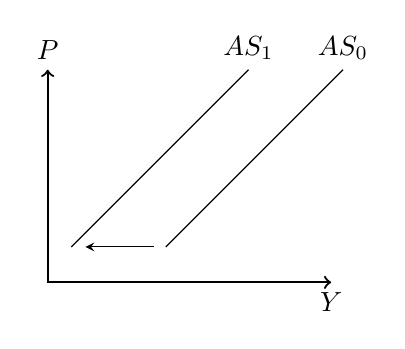
\begin{tikzpicture}[scale=0.3]	
	\draw[thick,<->] (0,9) node[above]{$P$}--(0,0) node[below right]{}--(12,0) node[below]{$Y$};
	\draw(1,1.5) -- (8.5,9) node[above]{$AS_1$};
	\draw(5,1.5) -- (12.5,9) node[above]{$AS_0$};
	\draw[stealth-] (1.6,1.5) -- (4.5,1.5) ;
	%		\draw (2,9) --(8.5,1.3) node[right]{$AD$};
	%		\draw(8,9)--(8,0) node[below]{$Y_f$};
	%		\draw[dashed](6.53,3.6)--(6.53,0) node[below] {$Y_e$};
\end{tikzpicture}
\end{center}
%		\end{minipage}

%\boxx{\textbf{Herleitung:} Die AS-Kurve beschreibt das aggregierte Angebot, welche sich durch die Lohnsetzung (wage setting), die Preissetzung (price setting) und die daraus resultierende natürliche Arbeitslosenquote (natural rate of unemployment) ergibt. Die Produktionsfunktion sowie die Kostenfunktion der Unternehmungen spielt hier eine Rolle. Dies wird im Kurs \textit{BWC 211 Volkswirtschaftslehre II Makroökonomie} genauer diskutiert.}

%\pbn
\paragraph{Factors influencing supply}
	Anything that increases production costs decreases supply at the same price. 
	\itex{
		\item Resources (input prices, availability) $\leftarrow$ pandemic, war, natural disasters, international politics, \dots.
		\item regulation $\leftarrow$ taxes, laws, subsidies, \dots.
		\item labor costs $\leftarrow$ unions, minimum wages, taxes, \dots 
		\item productivity $\leftarrow$ technology, research, management practices, \dots
		%\item \dots
	}

%
%\pbn
%\textbf{Verringern} sich die Produktionskosten, verschiebt sich die AS-Kurve nach \textbf{rechts}:
%\begin{center}
%	\begin{tikzpicture}[scale=0.3]	
%	\draw[thick,<->] (0,9) node[above]{$P$}--(0,0) node[below right]{}--(12,0) node[below]{$Y$};
%	\draw(1,1.5) -- (8.5,9) node[above]{$AS_0$};
%	\draw(5,1.5) -- (12.5,9) node[above]{$AS_1$};
%	\draw[-stealth] (1.6,1.5) -- (4.5,1.5) ;
%	%		\draw (2,9) --(8.5,1.3) node[right]{$AD$};
%	%		\draw(8,9)--(8,0) node[below]{$Y_f$};
%	%		\draw[dashed](6.53,3.6)--(6.53,0) node[below] {$Y_e$};
%\end{tikzpicture}
%\end{center}
%
%(\textbf{Erhöhen} sich die Produktionskosten, verschiebt sich die AS-Kurve nach \textbf{links}.)










\exex{Effects of the lockdown on equilibrium}{Discuss what effects the lockdown had on aggregate supply and demand in the economy. Sketch, the equilibrium of the AS and AD curves in a price-output diagram before the lockdown and after. Aim to describe the actual changes from GDP and the price level for Germany.
\begin{center}
	\includegraphics[width=.4\textwidth]{/home/sthu/Dropbox/hsf/pic/makro/deu}
\end{center}
}

\pbn
\solx{Effects of the lockdown on equilibrium}{

\textbf{AS-curve:} It can be assumed that the lockdown increased production costs (additional precautions at the workplace), or important production factors were not available (microprocessors were stuck in China, people were not allowed to work or were restricted, certain events were prohibited). Ergo: the AS curve should have shifted to the left due to the lockdown. Due to ongoing delivery problems of many inputs, it can be assumed that this shift persists.

\textbf{AD curve:} There was increased demand for individual groups of goods (toilet paper, noodles, hygiene), and demand was also boosted by government intervention and transfers (see: \websmall \url{https://www.esrb.europa.eu/home/search/coronavirus/countries/html/esrb.covidpmc_germany.en.html} (VAT reduction, short-time allowance, etc.). This would suggest a rightward shift of the AD curve. At the same time, however, demand for many goods has plummeted, especially for goods that require spatial mobility or human proximity (tourism, cars, restaurants, events, etc.). This would lead to a leftward shift of the AD curve. 
Overall, we initially assume that the demand-reducing effects dominated in the first few months. After some time, it could be assumed, demand returned to normal. This is consistent with the data from \autoref{fig:demanddeu}.

Two possible short-term scenarios:

%\pbn

\begin{minipage}{0.6\textwidth}
	1. Demand decreases a bit:
	
	\begin{center}
		\begin{tikzpicture}[scale=0.46]	
			\draw[thick,<->] (0,9) node[above]{$P$}--(0,0) node[below right]{}--(12,0) node[below]{$Y$};
			\draw(5,1) -- (12,9) node[above]{$AS^0$};
			\draw(1,1) -- (8,9)  node[above]{$AS^1$};
			\tkzDefPoint(6.6,2.9){A}
			\draw[dashed](6.6,2.9)--(6.6,0) node[below]{$Y^0$};
			\draw[dashed](6.6,2.9)--(0,2.9) node[left]{$P^0$};
			\draw (2,9) node[left]{$AD^0$} --(8,1) ;
			\draw (2,6) node[left]{$AD^1$} --(6,1) ;
			\tkzDefPoint(3.6,4){B}
			\foreach \n in {B, A}
			\node at (\n)[circle,fill,inner sep=1.5pt]{};
			\draw[dashed](3.6,4)--(3.6,0) node[below]{$Y^1$};
			\draw[dashed](3.6,4)--(0,4) node[left]{$P^1$};				
			%		\draw(8,9)--(8,0) node[below]{$Y_f$};
			%		\draw[dashed](6.53,3.6)--(6.53,0) node[below] {$Y_e$};
			\draw[-stealth] (6.6,-1) -- (3.6,-1) ;
			\draw[stealth-] (-2,4) -- (-2,2.9) ;
		\end{tikzpicture}
	\end{center}
	%\end{minipage}
	%\begin{minipage}{0.5\textwidth}
	
	2. Demand decreases a lot:
	
	\begin{center}
		\begin{tikzpicture}[scale=0.46]	
			\draw[thick,<->] (0,9) node[above]{$P$}--(0,0) node[below right]{}--(12,0) node[below]{$Y$};
			\draw(5,1) -- (12,9) node[above]{$AS^0$};
			\draw(1,1) -- (8,9)  node[above]{$AS^1$};
			\tkzDefPoint(6.6,2.9){A}
			\draw[dashed](6.6,2.9)--(6.6,0) node[below]{$Y^0$};
			\draw[dashed](6.6,2.9)--(0,2.9) node[left]{$P^0$};
			\draw (2,9) node[left]{$AD^0$} --(8,1) ;
			\draw (1,3) node[above]{$AD^1$} --(2.5,1) ;
			\tkzDefPoint(1.8,1.9){B}
			\foreach \n in {B, A}
			\node at (\n)[circle,fill,inner sep=1.5pt]{};
			\draw[dashed](1.8,1.9)--(1.8,0) node[below]{$Y^1$};
			\draw[dashed](1.8,1.9)--(0,1.9) node[left]{$P^1$};				
			%		\draw(8,9)--(8,0) node[below]{$Y_f$};
			%		\draw[dashed](6.53,3.6)--(6.53,0) node[below] {$Y_e$};
			\draw[-stealth] (6.6,-1) -- (1.8,-1) ;
			\draw[stealth-] (-2,1.9) -- (-2,2.9) ;
		\end{tikzpicture}
	\end{center}
\end{minipage}
\begin{minipage}{0.4\textwidth}
	In scenario 1, output decreases and prices \textbf{increase}.\.
	In scenario 2, output decreases more and prices \textbf{decrease}.
	\begin{center}
		\includegraphics[width=.8\textwidth]{/home/sthu/Dropbox/hsf/pic/makro/deu}
	\end{center}
\end{minipage}\bigskip

In the medium term, demand may have returned to the old level, in which case it would be stylized in the AS-AD model as follows:

\begin{center}
	\begin{tikzpicture}[scale=0.46]	
		\draw[thick,<->] (0,9) node[above]{$P$}--(0,0) node[below right]{}--(12,0) node[below]{$Y$};
		\draw(5,1) -- (12,9) node[above]{$AS^0$};
		\draw(1,1) -- (8,9)  node[above]{$AS^1$};
		\tkzDefPoint(6.6,2.9){A}
		\draw[dashed](6.6,2.9)--(6.6,0) node[below]{$Y^0$};
		\draw[dashed](6.6,2.9)--(0,2.9) node[left]{$P^0$};
		\draw (2,9) node[left]{$AD^0$} --(8,1) ;
		%		\draw (2,6) node[left]{$AD^1$} --(6,1) ;
		\tkzDefPoint(4.8,5.3){C}
		\tkzDefPoint(3.6,4){B}
		\foreach \n in {B, A, C}
		\node at (\n)[circle,fill,inner sep=1.5pt]{};
		\draw[dashed](3.6,4)--(3.6,0) node[below]{$Y^1$};
		\draw[dashed](4.8,5.3)--(4.8,0) node[below]{$Y^2$};
		\draw[dashed](3.6,4)--(0,4) node[left]{$P^1$};		
		\draw[dashed](4.8,5.3)--(0,5.3) node[left]{$P^2$};		
		%		\draw(8,9)--(8,0) node[below]{$Y_f$};
		%		\draw[dashed](6.53,3.6)--(6.53,0) node[below] {$Y_e$};
		\draw[-stealth] (3.6,-1.3) -- (4.8,-1.3) ;
		\draw[-stealth] (-2,4) -- (-2,5.3) ;
	\end{tikzpicture}
	%\begin{center}
	\includegraphics[width=.3\textwidth]{/home/sthu/Dropbox/hsf/pic/makro/deu}
	%\end{center}
\end{center}

}



\subsection{International data}
\begin{center}
\includegraphics[width=.7\textwidth]{/home/sthu/Dropbox/hsf/pic/makro/all}
\end{center}



\pbn
\subsection{Summary}

\itex{
\item Aggregate demand results from the interplay of supply and demand. 
\item Policymakers can take measures to mitigate the negative economic effects of exogenous shocks:
\itex{
	\item Increase government spending and cut taxes to boost consumption, investment and exports.
	\item Take away fears to improve consumption and investment.
	\item Reduce production costs by taking over production costs (short-time allowance, subsidized loans), reducing entrepreneurial risk (guarantees, insolvency law), promoting productivity (taking over research and development costs).
}
\item The AS-AD model can be helpful to understand, anticipate and analyze macroeconomic ratios.
}

\pbn

\exex{Comparing the financial crisis to the Corona crisis}{
Study the two graphs shown below and read \cite{Arnold2022Ist}, see:\ \websmall \url{https://www.bmwk.de/Redaktion/DE/Schlaglichter-der-Wirtschaftspolitik/2022/04/13-ist-krise-gleich-krise.html}.

Discuss how far the 2009 financial crisis differs from the 2020 Corona crisis in terms of aggregate supply and demand. In doing so, address the components of demand in both crises. Using the AS-AD model, explain why general price increases were largely absent in the financial crisis--despite expansionary fiscal and monetary policies--but prices rose in the corona crisis. 

\begin{center}
	\includegraphics[width=.9\textwidth]{/home/sthu/Dropbox/hsf/pic/makro/bip-2008-heute}
	%\end{center}
	%
	%\begin{center}
	\includegraphics[width=.9\textwidth]{/home/sthu/Dropbox/hsf/pic/makro/preisindizes-uebersicht}
\end{center}
}

\solx{Comparing the financial crisis to the Corona crisis}{
Please discuss that in class.	
}
